\chapter{OLFACTION AND VISION SENSING BASED ROSL ALGORITHM}\label{chap:fusion}

\section{Introduction}
Traditionally, ROSL research uses olfaction data for robot navigation. Olfaction data is typically represented as the concentration level of a chemical (e.g., alcohol), and wind sensing, i.e., wind speed and direction sensing. These data have inherently less information about the odor source location. In contrast, vision data can include much more information about the location of an odor source. Thus, vision is used by most complex animals for odor source localization. 
This chapter discusses the incorporation of vision sensing in ROSL. The works covered in this chapter were published as a journal article \cite{hassan2024robotic}.

\subsection{Background}\label{Subsec:fusionBackground}
% Background (Limitation of olfaction-only) and problem statement
Chapter~\ref{chap:olfaction} shows that an olfaction-based ROSL algorithm like the moth-inspired algorithm can successfully localize odor sources in simple real-world environments with uniform laminar airflow. However in environments with complex airflow or plume distribution, olfaction-only ROSL methods can struggle to reach the odor source. Thus, while cellular organisms and simple organisms without vision (e.g., nematodes) use olfaction-based OSL \cite{lockery2011computational}, complex animals utilize multi-modal-sensing for odor source localization.

Somatosensory sensing (i.e., tactile sensing) and thermal sensing are not commonly used for finding odor sources. Vision, however, is crucial for locating the odor source \cite{kuang2014smelling}. Many different animal groups utilize vision for OSL navigation, including invertebrates such as fruit flies \cite{frye2009visually}, mosquitoes \cite{van2015mosquitoes}, beetles \cite{l2015integration}, raptors \cite{potier2019sight}, mammals, etc. Typically, vision works in conjunction with olfaction for animals to precisely identify the odor source. When animals sense high odor concentrations, they initially use vision to search for potential odor source targets. If such targets are not directly visible, they rely on reasoning and olfaction to trace odor plumes and approach the odor source. The final confirmation of the odor source usually depends on vision. Thus, both vision and olfaction are essential modalities for odor source localization.

Similarly, a robot equipped with both olfaction- and vision-sensing capabilities (e.g., a camera and a chemical sensor) should locate an unknown odor source more efficiently compared to olfaction-only OSL navigation methods. However, compared to olfaction, vision data has multiple orders of complexity. Thus, while simple analytical methods can be used to extract useful information from olfaction sensor data, extracting useful information from raw pixel values will require machine-learning-based image processing. Indeed, machine learning breakthroughs of the last decade were initiated in response to vision processing challenges. For instance, the first breakthrough CNN-based `Perceptron' model \cite{krizhevsky2012imagenet} was designed to win the ImageNet vision processing competition in 2012. After 2012, every winning project of the ImageNet competition was machine-learning based.

\subsection{Related Research}\label{Subsec:DLROSL}
Machine-learning (ML)-based methods are increasingly employed in OSL experiments. Recent advancements include the use of Deep Neural Networks (DNNs) to predict gas leak locations from stationary sensor networks and the application of reinforcement learning for plume-tracing strategies. For example, Kim et al. \cite{kim2019source} trained a Recurrent Neural Network (RNN) to predict potential odor source locations using data from stationary sensor networks obtained through simulation. Hu et al. \cite{hu2019plume} developed a plume-tracing algorithm based on model-free reinforcement learning, employing the deterministic policy gradient to train an actor-critic network for Autonomous Underwater Vehicle (AUV) navigation. Wang et al. \cite{wang2021implementation} trained an adaptive neuro-fuzzy inference system (ANFIS) to address the OSL problem in simulations, though real-world validations are needed to confirm its effectiveness.

All of these approach processes olfactory data with machine learning models. In robotics, olfaction sensors often process the concentration level or detection-rate of a chemical (e.g., alcohol). These representations inherently contain limited information about the location of the odor source. Thus, it is unclear if more complex algorithms can extract the ever-increasing amount of information from the limited olfaction data. In addition, most DL-based methods discussed above are validated in virtual environments through simulated flow fields and plume distributions, highlighting the need for real-world implementations to validate their effectiveness.

\subsection{Objectives}\label{Subsec:fusionObjectives}
This project diverges from the existing OSL navigation methods by utilizing both robotic vision and olfaction in searching for the odor source location. Olfaction-Only navigation methods often depend on airflow direction to locate the odor source, which can result in failure in turbulent airflow environments. Vision sensing can enable the robot to identify the plume source location within its visual field and approach it directly. Since visual sensing is not influenced by airflow, combining it with Olfaction-Based Navigation can help the robot better locate the odor source in turbulent airflow conditions. The core of this project is to train a deep-learning-based vision processor and to design an algorithm that integrates both vision and olfaction sensing for locating an unknown odor source location.
The objectives of this project are:
\begin{itemize}
\item to introduce vision as an additional sensing modality for ROSL. Extracting information from the vision required training of a deep-learning-based computer vision model;
\item to develop a multi-modal Vision and Olfaction Fusion Navigation algorithm with Obstacle-Avoid Navigation capabilities for ROSL tasks;
\item to compare the search performance of Olfaction-Only and Vision-Only Navigation algorithms with the proposed Vision and Olfaction Fusion Navigation algorithm in a real-world search environment with obstacles and turbulent airflow setups.    
\end{itemize}

%%%%%%%%%%%%%%%%%%%%%%%%%%%%%%%%%%%%%%%%%%%%%%%%%%%%%%%%%%%%%%%%%%%%%%%%%%%%%%

\section{Methodology}
The project introduces an efficient sensor fusion algorithm that combines vision and moth-inspired olfaction-based navigation for ROSL. To augment the capabilities of this navigation algorithm, we added obstacle avoidance capability with it. Details of the olfaction model can be found in chapter~\ref{chap:olfaction}, the deep-learning-based vision model is discussed in subsection~\ref{Subsec:fusion_vision-model}, the obstacle avoidance behavior is discussed in subsection~\ref{Subsec:obstacle-avoid}, and the proposed fusion algorithm is discussed in subsection~\ref{Subsec:fusionROSL}.

\subsection{Deep-learning-based Vision Processing Model}\label{Subsec:fusion_vision-model}
The proposed Vision-Based Navigation relies on deep-learning-based computer vision techniques. Specifically, we train a deep-learning-based object detection model, namely YOLOv7, to identify vapors emitted from the odor source. Vapors are a common and distinct feature of the odor source object, such as smoke from fire sources or chemical plumes from chemical leaks, or hydrothermal vents. It is important to note that if the odor source lacks a distinct plume feature (i.e., transparent vapors), the robot can still locate the odor source using the Olfaction-Based Navigation behavior of the proposed Vision and Olfaction Fusion algorithm. Furthermore, we provide a real-world performance comparison between Olfaction-Based Navigation, Vision-Based Navigation, and the proposed navigation algorithms.

\begin{figure}[h] %% figure

\ \\
\vspace*{-.18in}

\begin{center}
    \subfigure{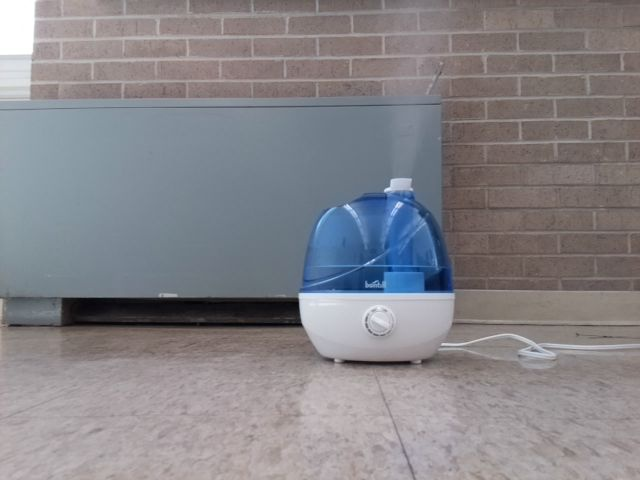
\includegraphics[width=0.5\columnwidth]{Main/Figure/visionTrainingData1.jpg}}\hspace*{0.04in}
    \subfigure{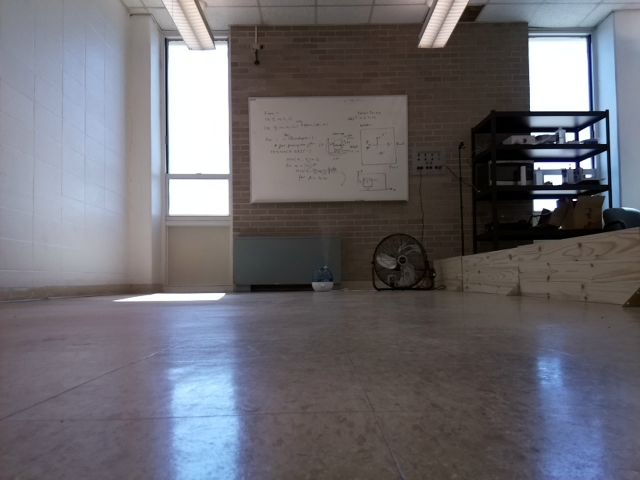
\includegraphics[width=0.5\columnwidth]{Main/Figure/visionTrainingData2.jpg}}\hspace*{0.04in}
\end{center}
\vspace{-.1in}

\caption
{Two sample frames that include humidifier odor plumes in different lighting and spatial conditions. The frames are sampled out of the total 243 frames used for training the vision model. All of the frames were captured by the Turtlebot robot in the experiment area.}
%\end{singlespace}
\label{fig:visionModelTrainingData}
\end{figure}

To generate training images for the vision model, we extracted 243 observation frames with a resolution of $640 \times 480$ while the Turtlebot was approaching the odor plumes from various angles, distances, and lighting conditions. Figure~\ref{fig:visionModelTrainingData} shows two sample frames used for training the vision model. Roboflow \cite{ciaglia2022roboflow} was used for labeling the images. This data was augmented to increase volume and was divided into training, validation, and testing datasets for model training. We used the 'Ultralytics' implementation of the YOLOv7 model, which required two hyper-parameter inputs. Epoch size of 100 and batch size of 16 resulted in a training accuracy of 98\%, and a testing accuracy of 93\%.

The implemented vision model detects if there is an odor source in the current visual frame, and if it is in the left or right part of the visual frame. In the implementation, the trained model returns the coordinates of the target object bounding box if it detects visible plume in the current visual frame. If the model detects a plume, the robot continues moving forward (i.e., $v_c=0.5$ m/s) and checks if the mid-horizontal coordinate of the bounding box is greater or less than the mid-horizontal coordinate value of the visual frame. The model took on average $1 s$ to produce output using cuda cores of RTX3060 mobile GPU of the remote computer. Thus we pass every $sr^th$ frame to the model, where $sr$ is the set value for the sensor refresh rate.

Equation~(\ref{eqn:vision_heading}) calculates the robot's heading
\begin{equation}
  \omega_c =
    \begin{cases}
       1 & \text{$0.5$ m/s if $c<\dfrac{w}{2}$}\\
      2 & \text{$-0.5$ m/s if $c>\dfrac{w}{2}$},
    \end{cases}
\label{eqn:vision_heading}
\end{equation}
where $c$ represents the horizontal midpoint of the bounding box and $w$ is the horizontal resolution of the captured image. If the bounding box is located in the left half of the image (i.e., $c < \dfrac{w}{2}$), the robot rotates left (i.e., $\omega_c = 0.5$ rad/s) to align with the plume. Otherwise, it rotates right (i.e., $\omega_c = -0.5$ rad/s) to face the plume.

\subsection{Obstacle-Avoid Navigation Behavior}\label{Subsec:obstacle-avoid}
The `Obstacle-Avoid Navigation' behavior is activated when the robot approaches an obstacle within the search environment, directing it to navigate around and avoid the obstacles. This project utilizes a Laser Distance Sensor (LDS) to sense obstacles in the surrounding area.

The proposed obstacle-avoidance behavior was derived empirically in our navigation setup. The main concept of this behavior is to determine the relative location of obstacles to the robot and command the robot to move around them. It tries to make a minimum angular change to the active direction while avoiding obstacles. The fusion algorithm avoided obstacles situated in less than $1 m$ in front - ($laser[0]$), $0.75 m$ in slightly left and right sides - ($laser[45]$) and ($laser[315]$), $0.5 m$ in left and right sides - ($laser[90]$) and ($laser[270]$). Figure~\ref{fig:laser_distance_sensing} depicts the laser distance sensing. 

\begin{figure}[h!] %% figure

\ \\
\vspace*{-.18in}

\begin{center}
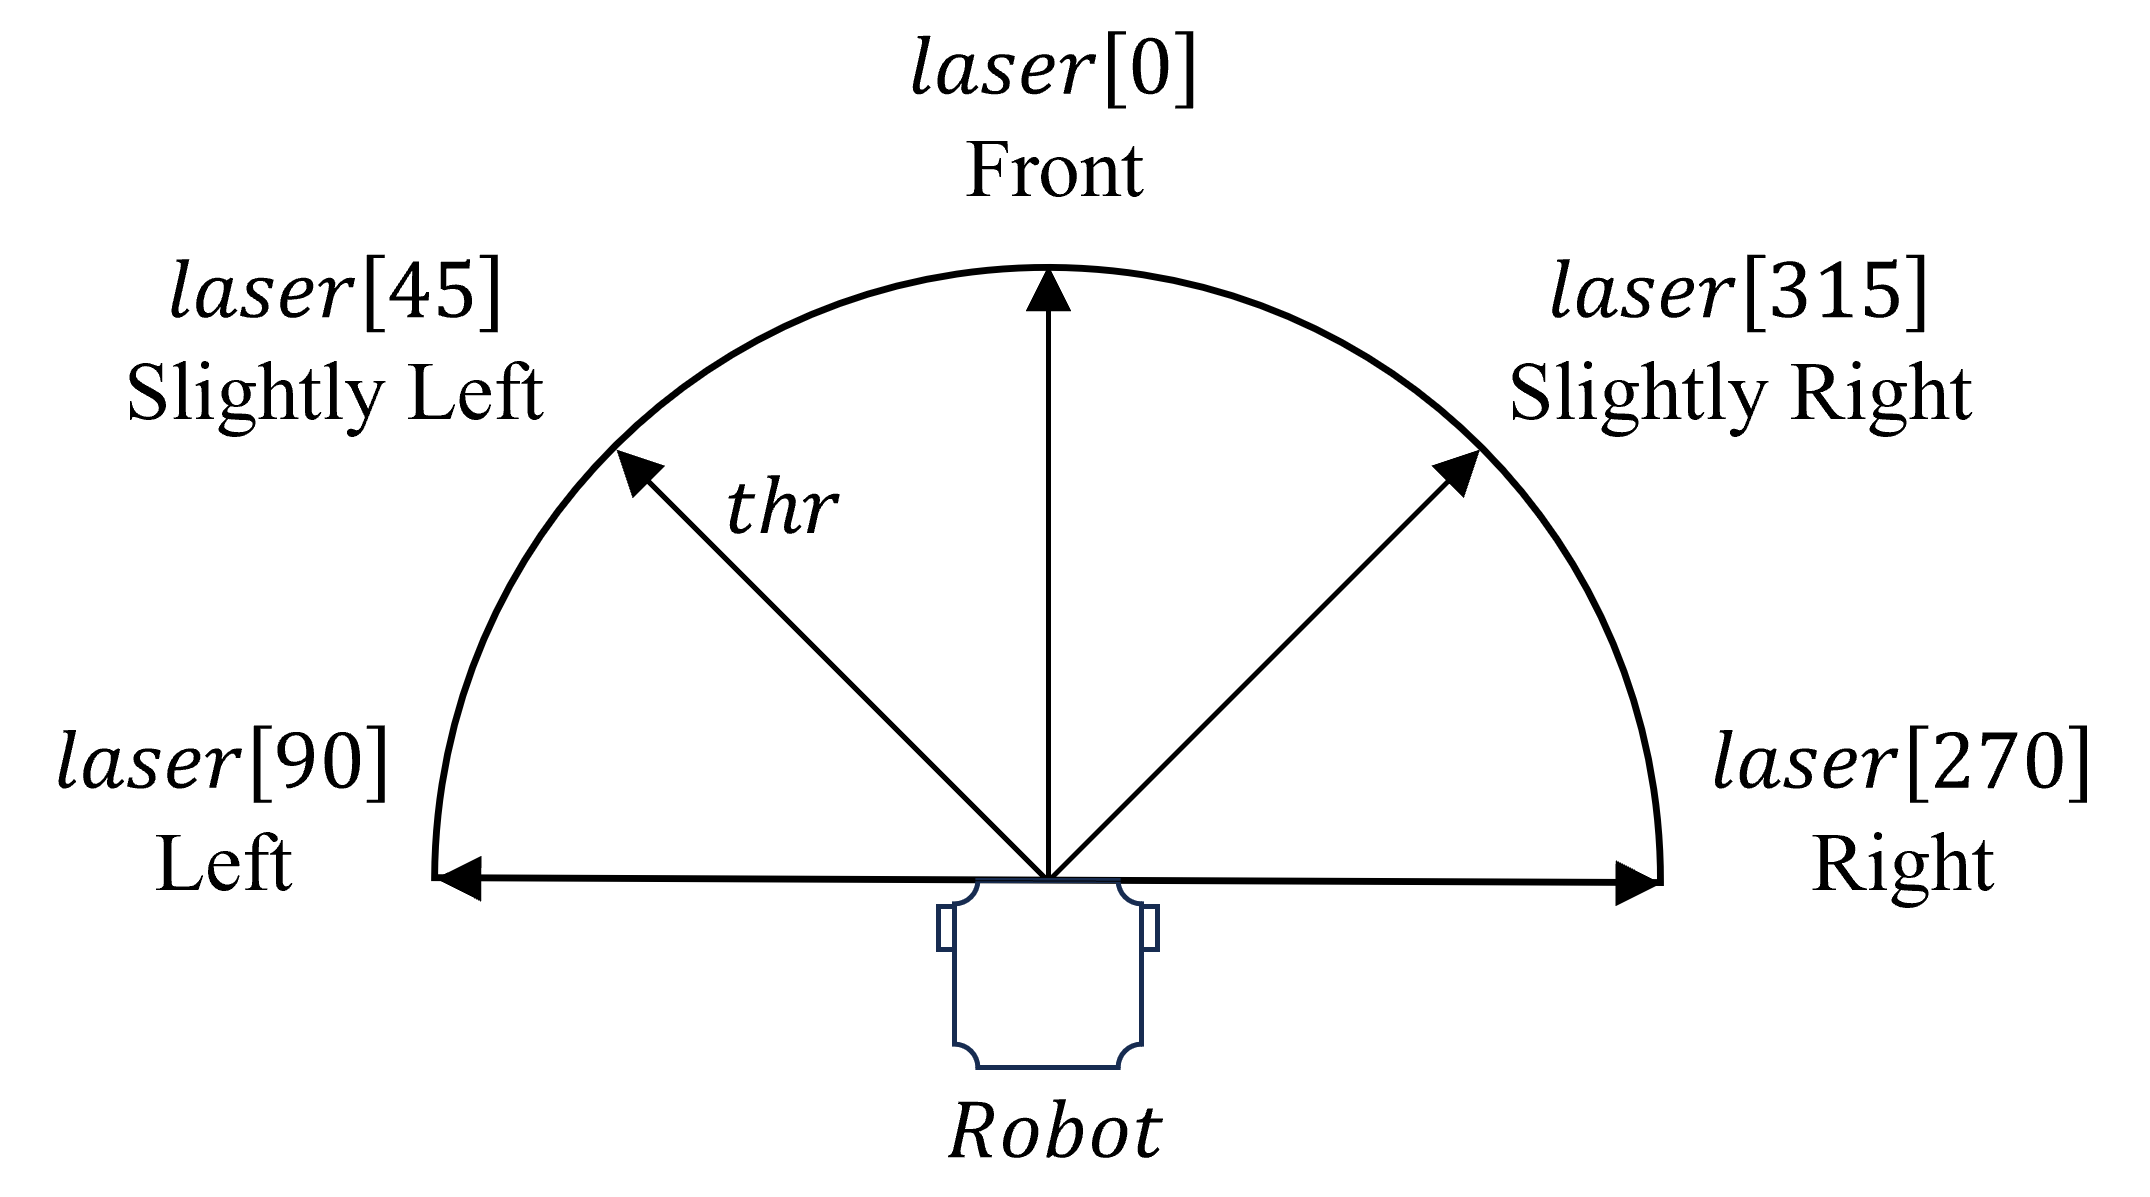
\includegraphics[width=0.7\columnwidth]{Main/Figure/robot_laserReadings.png}\hspace*{0.04in}
\end{center}
\vspace{-.1in}

\caption
{Five directions in the robot's laser distance sensing, including Left, Slightly Left, Front, Slightly Right, and Right. $laser[x]$ denotes the distance between the robot and the object at the angle $x$, which is measured from the onboard laser distance sensor.}
%\end{singlespace}
\label{fig:laser_distance_sensing}
\end{figure}


\begin{algorithm}[h!]
\caption{`Obstacle-Avoid Navigation' Behavior}\label{alg:obstacle-avoid}
\begin{algorithmic}[1]
\State Set robot linear velocity as $v_c=0.6$ m/s
\State Set robot angular velocity as $\omega_c=0$ rad/s
\If{$laser[0] > thr$}
    \State $\omega_{c}=0$ rad/s
\Else
    \State $v_c=0$ m/s and $\omega_{c}=0$ rad/s
    \If{$(laser[45]>thr)\lor (laser[315]>thr)$}
        \If{$laser[45]>laser[315]$}
            \State $\omega_{c}=0.5$ rad/s
        \Else
            \State $\omega_{c}=-0.5$ rad/s
        \EndIf
    \ElsIf{$(laser[90]>thr)\lor (laser[270]>thr)$}
        \If{$laser[90]>laser[270]$}
            \State $\omega_{c}=0.5$ rad/s
        \Else
            \State $\omega_{c}=-0.5$ rad/s
        \EndIf
    \Else
        \State $v_c=-0.5$ m/s
    \EndIf
\EndIf

\end{algorithmic}
\end{algorithm}

In the `Obstacle-Avoid Navigation' behavior \ref{alg:obstacle-avoid}, the robot continually checks for a clear path ahead, i.e., $laser[0] > thr$ (where $thr$ is the threshold for obstacle detection, set at 0.75 m in this work). If the path is clear, the robot moves forward without angular velocity, $\omega_{c} = 0$ rad/s. If the front is blocked, the robot stops and checks for clearance in Slightly Left or Slightly Right ($(laser[45] > thr) \lor (laser[315] > thr)$) directions. If either direction is clear, the robot compares the clearance between Slightly Left and Slightly Right and rotates left (i.e., $\omega_{c} = 0.5$ rad/s) or right (i.e., $\omega_{c} = -0.5$ rad/s) toward the greater clearance. If there is no clearance in either Slightly Left or Slightly Right, the robot checks for a clear path to the Left or Right ($(laser[90] > thr) \lor (laser[270] > thr)$). If a clear path exists, the robot compares the clearance between Left and Right ($laser[90] > laser[270]$) and rotates left ($\omega_{c} = 0.5$ rad/s) or right ($\omega_{c} = -0.5$ rad/s) toward the greater clearance. If all five directions are blocked, the robot moves backward ($v_c = -0.5$ m/s) to escape the dead end.

It is important to note that the proposed navigation algorithm does not have access to the global map of the search environment, the locations of obstacles, or the destination odor source. Therefore, planning-based obstacle avoidance algorithms such as the Artificial Potential Field algorithm \cite{al2022new}, A* algorithm \cite{xiang2022combined}, and Dijkstra algorithm \cite{luo2020surface} are not applicable to our problem. In such partially observable environments, using discrete behavior control is the best option. A similar approach was used in \cite{kahn2021badgr}. Compared to classic motion-planning algorithms (e.g., Dijkstra, A*, APF), our proposed obstacle avoidance algorithm has the following advantages:
\begin{itemize}
    \item It does not rely on prior knowledge of the global map, the location of obstacles, or the destination;
    \item Compared to most deep-learning-based navigation planners, it requires less inference time.
\end{itemize}


\subsection{Vision and Olfaction Fusion Algorithm}\label{Subsec:fusionROSL}

\begin{figure}[h] %% figure

\ \\
\vspace*{-.18in}

\begin{center}
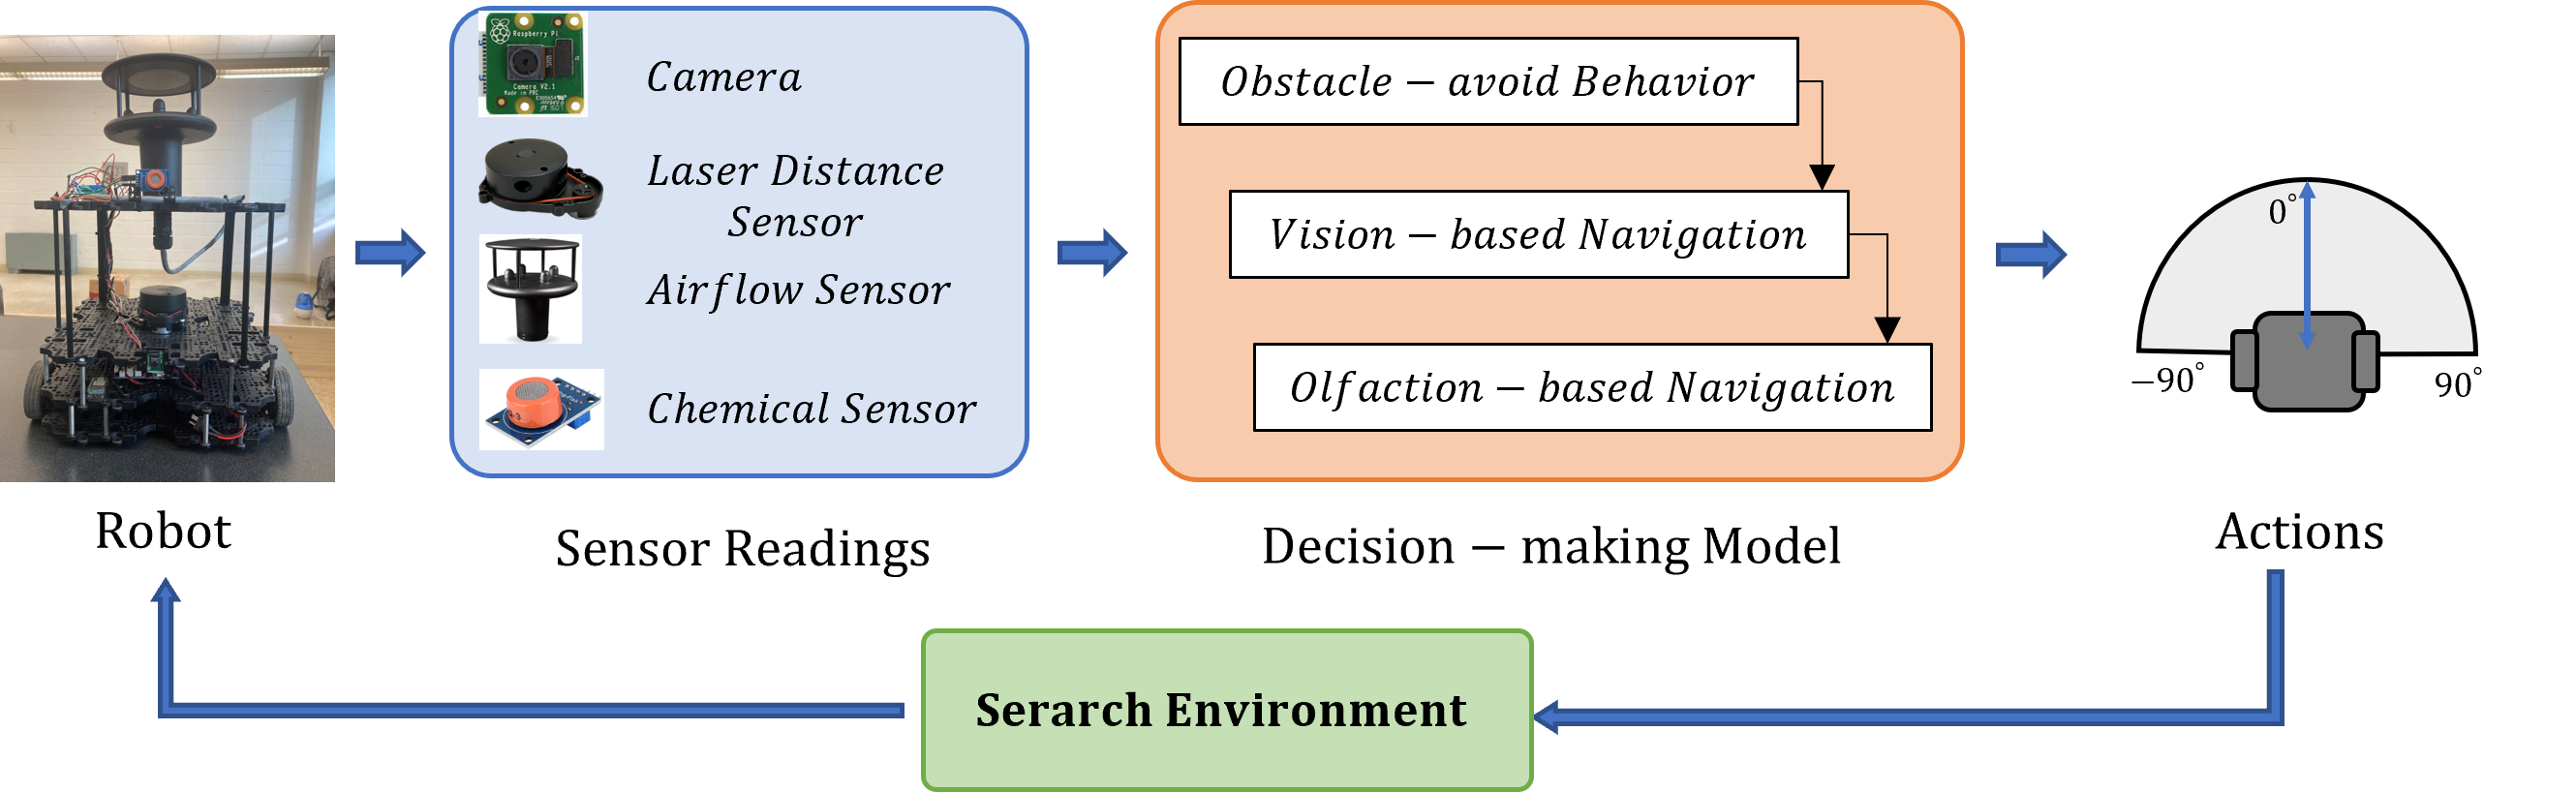
\includegraphics[width=0.7\columnwidth]{Main/Figure/OSL Model.png}\hspace*{0.04in}
\end{center}
\vspace{-.1in}

\caption
{Flow diagram of the proposed method for the OSL experiment. We employed the Turtlebot3 robot platform, outfitting it with a camera, Laser Distance Sensor, airflow sensor, chemical sensor, and other essential components. The robot uses three navigation behaviors—Obstacle-Avoid Navigation, Vision-Based Navigation, and Olfaction-Based Navigation—to determine its heading and linear velocity.}
%\end{singlespace}
\label{fig:osl_model}
\end{figure}

The proposed fusion algorithm should be able to navigate in an environment with obstacles to localize odor sources in both simple laminar and complex turbulent airflow environments. Figure~\ref{fig:osl_model} illustrates the proposed method, showcasing the developed robot platform equipped with vision and olfaction sensors. The vision sensors include a camera, while the olfaction sensors consist of a chemical detector and an anemometer. Additionally, the platform features a Laser Distance Sensing (LDS) for detecting obstacles. Vision sensor data is used by the trained YOLOv7 model to detect the presence of an odor source in the current visual frame. The output from the vision model and the raw olfaction data are transmitted to the fusion ROSL model. Based on the inputs, the model analytically determines a behavior - Obstacle-Avoid Navigation, Vision-Based Navigation, or Olfaction-Based Navigation - which is again subdivided into moth-inspired crosswind and upwind navigation. Based on the active search behavior, the algorithm calculates linear and angular heading commands. The robot then executes the heading command, gathers new sensor data at its new location, transmits it to the remote computer, and receives a new heading command - this cycle repeats until the odor source is found.

\begin{figure}[h!] %% figure

\ \\
\vspace*{-.18in}

\begin{center}
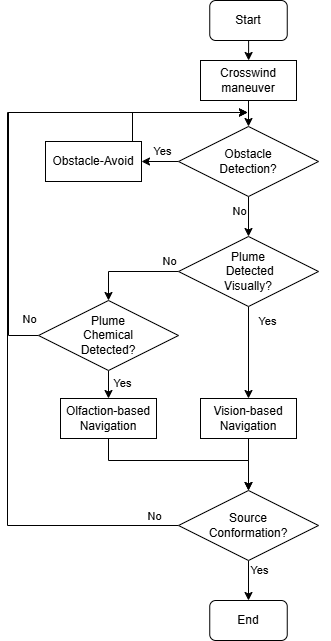
\includegraphics[width=0.5\columnwidth]{Main/Figure/FusionFlowDiagram.png}\hspace*{0.04in}
\end{center}
\vspace{-.1in}

\caption
{The flow diagram of the proposed OSL algorithm. There are four navigation behaviors, including `Crosswind maneuver', `Obstacle-Avoid Navigation', `Vision-Based Navigation', and `Olfaction-Based Navigation'.}
%\end{singlespace}
\label{fig:flow_diagram}
\end{figure}

Figure~\ref{fig:flow_diagram} illustrates the flow diagram of the proposed navigation algorithm. The fusion algorithm first checks for obstacles in the surrounding region with LDS. If there is any obstacle in the surrounding area, the algorithm activates the `Obstacle-Avoid Navigation' behavior, maneuvering the robot around the obstacles. If there are no obstacles in the surrounding area, the algorithm checks if it can sense sufficient plume concentration or valid visual detection of the plume source. In the absence of such detection, the algorithm activates the `Crosswind maneuver' behavior, moving the robot crosswind to increase the chance of detecting chemical or visual cues. During this, if a valid visual detection is obtained, the algorithm activates 'Vision-based' navigation behavior, directly moving the robot toward the odor source. If there is no visual detection, but sufficient chemical detection is recorded, the algorithm activates 'Olfaction-based' navigation behavior, sending the robot upwind. This cycle is repeated until the robot moves in the vicinity of the odor source, and the algorithm declares the source, marking the end of the search.

%%%%%%%%%%%%%%%%%%%%%%%%%%%%%%%%%%%%%%%%%%%%%%%%%%%%%%%%%%%%%

\section{Experiment}\label{Sec:fusionExperiment}

The focus of the experiment was to analyze and compare the navigation patterns of olfaction-only and vision-only navigation separately, and then then to compare the performance and navigation pattern of the fusion navigation model.

% ROSL navigation task
\subsection{Navigation Task}\label{Subsec:fusionNavigationTask}
\begin{figure}[h!] %% figure
\ \\
\vspace*{-.18in}
\begin{center}
\subfigure[Search Area]{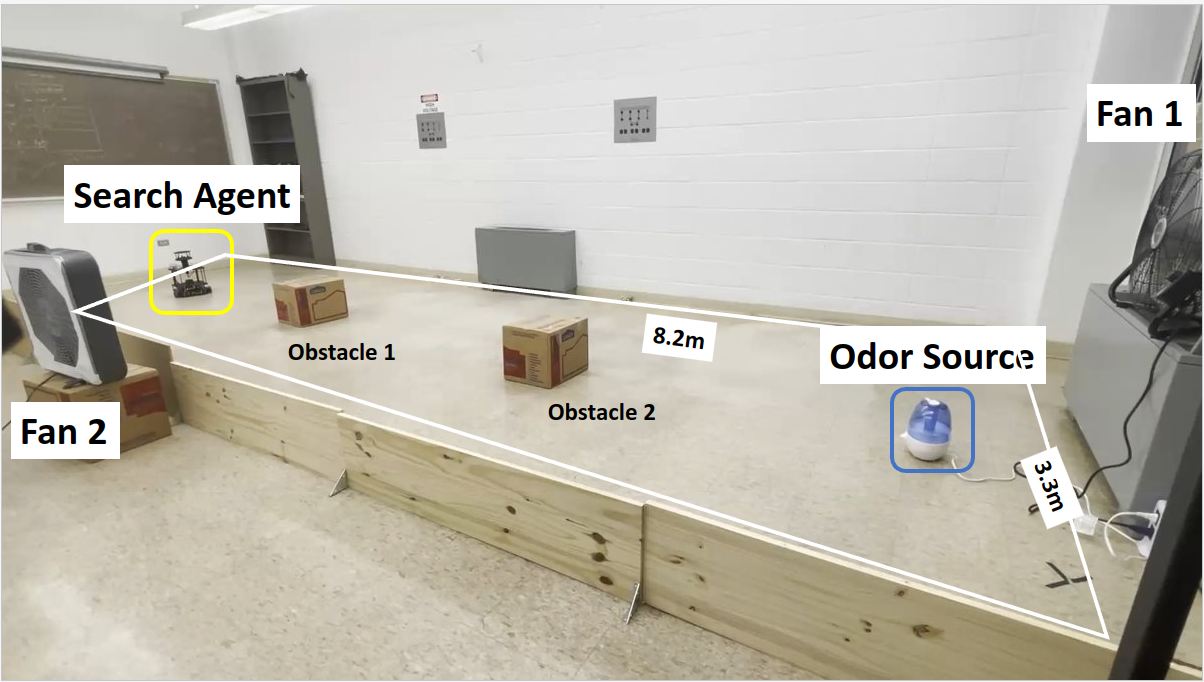
\includegraphics[width=0.55\columnwidth]{Main/Figure/Search area.png}}\hspace*{0.04in}
\subfigure[Mobile Robot]{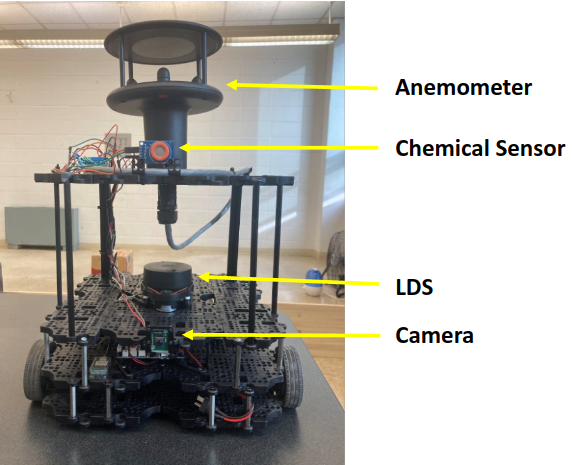
\includegraphics[width=0.4\columnwidth]{Main/Figure/mobile_robot.png}}\hspace*{0.04in}
\end{center}
\vspace{-.1in}

\caption
{(a) The experimental setup. The robot is initially placed in a downwind area with the objective of finding the odor source. A humidifier loaded with ethanol is employed to generate odor plumes. Two electric fans are placed perpendicularly to create artificial wind fields. Two obstacles are placed in the search area. {(b)} The Turtlebot3 waffle pi mobile robot is used in this work. In addition to the camera and Laser Distance Sensor, the robot is equipped with a chemical sensor and an anemometer for measuring chemical concentration, wind speeds, and directions.}
%\end{singlespace}
\label{fig:search_area_real}
\end{figure}

\begin{figure}[h!] %% figure
\ \\
\vspace*{-.18in}
\begin{center}
\subfigure[Laminar environment]{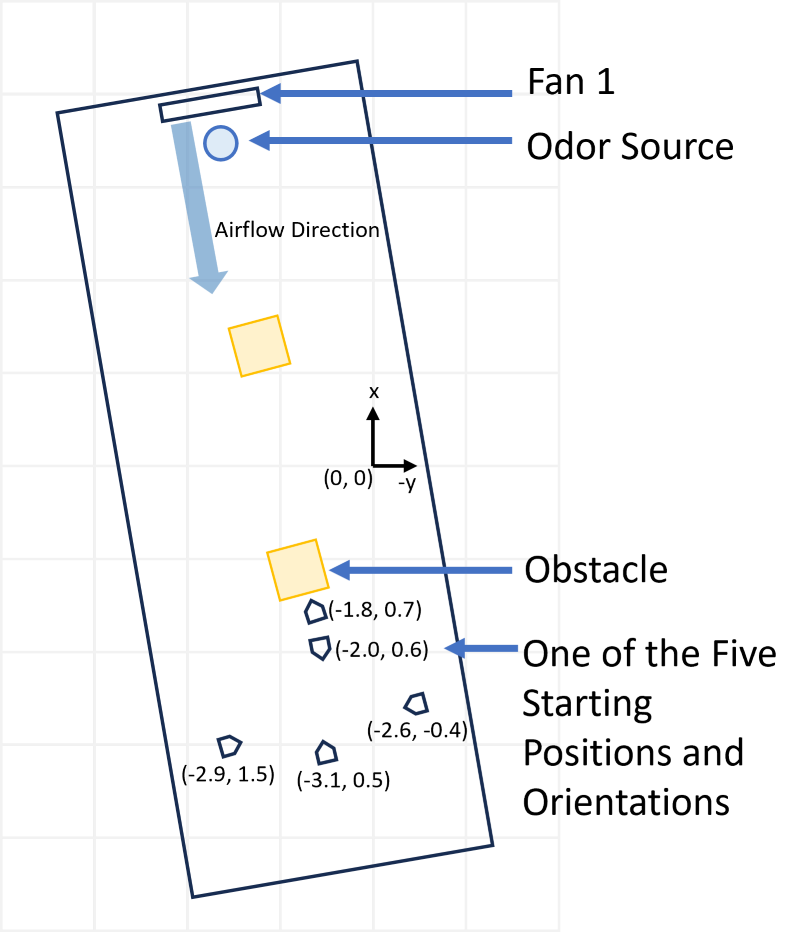
\includegraphics[width=0.4\columnwidth]{Main/Figure/Search Area Schematic Diagram e1.png}}\hspace*{0.04in}
\subfigure[Turbulent environment]{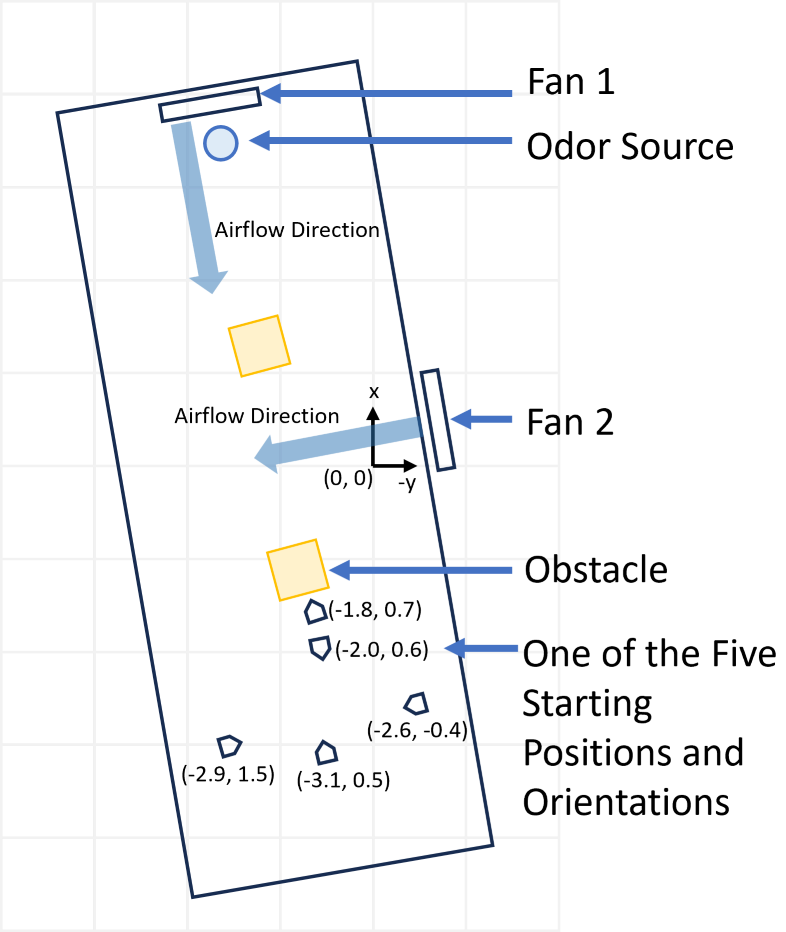
\includegraphics[width=0.4\columnwidth]{Main/Figure/Search Area Schematic Diagram e2.png}}\hspace*{0.04in}
\end{center}
\vspace{-.1in}

\caption
{The schematic diagram of the search area with e1$-$laminar airflow setup. The five robot starting positions are used for testing the performance of the Olfaction-Based Navigation, Vision-Based Navigation, and Vision and Olfaction Fusion Navigation tests. {(b)} The schematic diagram of the search area with e2$-$turbulent airflow setup.}
\label{fig:demonstration}
\end{figure}

The ROSL navigation task is similar to the one discussed in section~\ref{Sec:olfactionExperiment}. The robot will be initiated at one of the pre-determined starting positions in the search area, and it use the sensor data to navigate to the odor source location. Figure~\ref{fig:search_area_real}(a) shows the two-dimensional 8.2 m $\times$ 3.3 m search area, and the Figure~\ref{fig:search_area_real}(b) shows the robot platform. The robot platform development was detailed in subsection~\ref{Subec:OSLHardware}.

Two obstacles were placed in the search area to simulate a complex real-world search environment. The obstacles served some important purposes: 1) to test obstacle avoidance capability, 2) to block initial plume vision from the robot, 3) to further impact airflow, etc. The fans were placed to create both laminar and turbulent airflow environments in the search area. In laminar flow environments, only one fan was employed, and it was placed behind the odor source to accelerate the plume diffusion rate and create a unified wind direction field as presented in Figure\ref{fig:demonstration}{(a)}). In turbulent flow environments, we used two fans and placed them at perpendicular positions to create a mixed and turbulent wind field (as presented in Figure \ref{fig:demonstration}{(b)}).


\subsection{Reference Olfaction-only and Vision-only Algorithms}\label{subsec:fusionReferenceAlgorithms}

We designed two different navigation algorithms - only olfaction sensing-based navigation algorithm, and only vision sensing-based navigation algorithm. The purpose is to compare their navigation pattern and ROSL success rates. They were further compared with the proposed Fusion Navigation Algorithm.

\begin{figure}[h!] %% figure
\ \\
\vspace*{-.18in}
\begin{center}
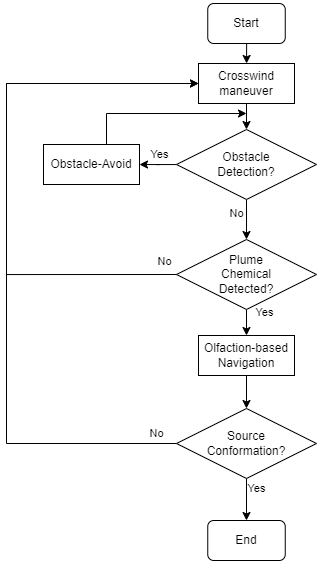
\includegraphics[width=0.4\columnwidth]{Main/Figure/OlfactionFlowDiagram.png}\hspace*{0.04in}
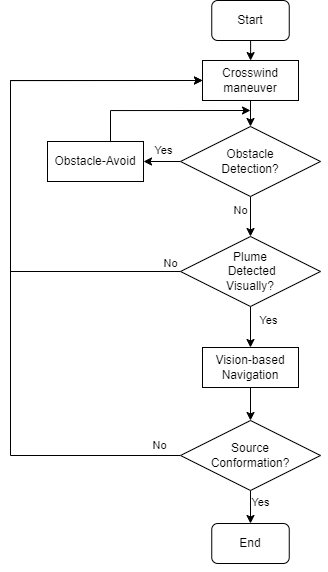
\includegraphics[width=0.4\columnwidth]{Main/Figure/VisionFlowDiagram.png}\hspace*{0.04in}
\end{center}
\vspace{-.1in}

\caption
{(a) The flow diagram of the Olfaction-Only Navigation algorithm. There are three navigation behaviors, including `Crosswind maneuver', `Obstacle-Avoid Navigation', and `Olfaction-Based Navigation'. {(b)} The flow diagram of the Vision-Only Navigation algorithm. There are three navigation behaviors, including `Crosswind maneuver', `Obstacle-Avoid Navigation', and `Vision-Based Navigation'.}
\label{fig:comparisonAlgorithm}
\end{figure}


Figure~\ref{fig:comparisonAlgorithm}(a) shows the Olfaction-Only Navigation algorithm. The algorithm first checks for obstacles in the surrounding region with LDS. If there is any obstacle in the surrounding area, the algorithm activates the `Obstacle-Avoid Navigation' behavior, maneuvering the robot around the obstacles. If there are no obstacles in the surrounding area, the algorithm checks if it can sense sufficient plume concentration. In the absence of such detection, the algorithm activates the `Crosswind maneuver' behavior, moving the robot crosswind to increase the chance of detecting chemical cues. If sufficient chemical detection is recorded, the algorithm activates 'Olfaction-based' navigation behavior, sending the robot upwind. This cycle is repeated until the robot moves in the vicinity of the odor source, and the algorithm declares the source, marking the end of the search.

Figure~\ref{fig:comparisonAlgorithm}(b) shows the Vision-Only Navigation algorithm. The algorithm first checks for obstacles in the surrounding region with LDS. If there is any obstacle in the surrounding area, the algorithm activates the `Obstacle-Avoid Navigation' behavior, maneuvering the robot around the obstacles. If there are no obstacles in the surrounding area, the algorithm checks if it can sense valid visual detection of the plume source. In the absence of such detection, the algorithm activates the `Crosswind maneuver' behavior, moving the robot crosswind to increase the chance of detecting visual cues. During this, if a valid visual detection is obtained, the algorithm activates 'Vision-based' navigation behavior, directly moving the robot towards the odor source. This cycle is repeated until the robot moves in the vicinity of the odor source, and the algorithm declares the source, marking the end of the search.

\subsection{Evaluation Metric}\label{subsec:fusionEvaluationMetric}
% Performance metric (type/number of tests, analysis and success matric)
% Real-world experimentation setup
These three algorithms were tested in two airflow environments, including the e1---laminar airflow environment and the e2---turbulent airflow environment. Thus, a total of six experimental setups were designed, i.e., three navigation methods in two airflow environments, to test the effectiveness of the proposed fusion model. Five experimental runs were conducted for each of the six experimental setups, totaling 30 trial runs. We used the same five starting positions to initialize the test runs for the three algorithms for comparability. Figure~\ref{fig:demonstration} shows the five starting positions and the two airflow setups for the experimental runs. The success rates of the three algorithms is compared to validate the effectiveness of the proposed fusion navigation algorithm.


%%%%%%%%%%%%%%%%%%%%%%%%%%%%%%%%%%%%%%%%%%%%%%%%%%%%%%%%%%%%%%%%%%%%%%%%%%%%%%55

\section{Results and Discussion}\label{Sec:fusionResult}
% trajectory graphs and result tables
% conclusion

\begin{table}[h!]

\ \\

\caption{Search time of the Vision-Only, Olfaction-Only, and Proposed Vision and Olfaction Fusion Navigation algorithms. The notation (-) indicates that the search time is beyond the limit, which is 200 seconds in this work.}
\label{tab:expeiment_result}
\ \\
\centerline{
\begin{tabular}{|c|c|c|c|c|}
\hline
\textbf{\begin{tabular}[c]{@{}c@{}}Airflow\\ Environment\end{tabular}} & \textbf{\begin{tabular}[c]{@{}c@{}}Robot\\ Initial\\ Position\\ (x, y), \\ Orientation\\ (z, w)\end{tabular}} & \textbf{\begin{tabular}[c]{@{}c@{}}Olfaction-\\ Only\\ Navigation\\ Algorithm\\ (s)\end{tabular}} & \textbf{\begin{tabular}[c]{@{}c@{}}Vision-Only\\ Navigation\\ Algorithm\\ (s)\end{tabular}} & \textbf{\begin{tabular}[c]{@{}c@{}}Vision and\\ Olfaction\\ Fusion\\ Navigation\\ Algorithm\\ (s)\end{tabular}} \\ \hline
\multirow{5}{*}{Laminar}                                               & \begin{tabular}[c]{@{}c@{}}(−2.9, 1.5),\\ (−0.6, 1.0)\end{tabular}                                            & \textbf{63.1}                                                                                     & -                                                                                           & 63.9                                                                                                            \\ \cline{2-5} 
                                                                       & \begin{tabular}[c]{@{}c@{}}(−3.1, 0.5),\\ (0.0, 35.0)\end{tabular}                                            & 71.3                                                                                              & 149.3                                                                                       & \textbf{69.9}                                                                                                   \\ \cline{2-5} 
                                                                       & \begin{tabular}[c]{@{}c@{}}(−2.6, −0.4),\\ (0.7, 0.7)\end{tabular}                                            & 74.3                                                                                              & -                                                                                           & \textbf{67.5}                                                                                                   \\ \cline{2-5} 
                                                                       & \begin{tabular}[c]{@{}c@{}}(−2.0, 0.6),\\ (1.0, −0.1)\end{tabular}                                            & \textbf{73.8}                                                                                     & -                                                                                           & 75.7                                                                                                            \\ \cline{2-5} 
                                                                       & \begin{tabular}[c]{@{}c@{}}(−1.8, 0.7),\\ (0.0, 0.1)\end{tabular}                                             & \textbf{59.1}                                                                                     & -                                                                                           & 61.1                                                                                                            \\ \hline
\multirow{5}{*}{Turbulent}                                             & \begin{tabular}[c]{@{}c@{}}(−2.9, 1.5),\\ (−0.6, 1.0)\end{tabular}                                            & -                                                                                                 & -                                                                                           & \textbf{64.0}                                                                                                   \\ \cline{2-5} 
                                                                       & \begin{tabular}[c]{@{}c@{}}(−3.1, 0.5),\\ (0.0, 35.0)\end{tabular}                                            & -                                                                                                 & -                                                                                           & \textbf{113.1}                                                                                                  \\ \cline{2-5} 
                                                                       & \begin{tabular}[c]{@{}c@{}}(−2.6, −0.4),\\ (0.7, 0.7)\end{tabular}                                            & 196.4                                                                                             & -                                                                                           & \textbf{130.7}                                                                                                  \\ \cline{2-5} 
                                                                       & \begin{tabular}[c]{@{}c@{}}(−2.0, 0.6),\\ (1.0, −0.1)\end{tabular}                                            & -                                                                                                 & 102.8                                                                                       & \textbf{131.9}                                                                                                  \\ \cline{2-5} 
                                                                       & \begin{tabular}[c]{@{}c@{}}(−1.8, 0.7),\\ (0.0, 0.1)\end{tabular}                                             & 72.3                                                                                              & -                                                                                           & \textbf{68.5}                                                                                                   \\ \hline
\end{tabular}}

\ \\
\vspace{-.1in}

\end{table}


\begin{table}[h]

\ \\

\caption{Result statistics, i.e., success rate and average search time of Vision-Based Navigation, Olfaction-Based Navigation, and the Proposed Vision and Olfaction Fusion Navigation Algorithms.}
\label{tab:expeiment_stat}
\ \\
\centerline{
\begin{tabular}{|c|c|c|c|c|}
\hline
\textbf{\begin{tabular}[c]{@{}c@{}}Navigation\\ Algorithm\end{tabular}}                     & \textbf{\begin{tabular}[c]{@{}c@{}}Airflow\\ Environment\end{tabular}} & \textbf{\begin{tabular}[c]{@{}c@{}}Success\\ Rate\end{tabular}} & \textbf{\begin{tabular}[c]{@{}c@{}}Avg.\\ Search\\ Time (s)\end{tabular}} & \textbf{\begin{tabular}[c]{@{}c@{}}Avg.\\ Travelled\\ Dist. (m)\end{tabular}} \\ \hline
\multirow{2}{*}{\textbf{Olfaction-only}}                                                    & \textbf{Laminar}                                                       & \textbf{5/5}                                                    & 68.3                                                                      & \textbf{6.1}                                                                  \\ \cline{2-5} 
                                                                                            & \textbf{Turbulent}                                                     & 2/5                                                             & 134.4                                                                     & 9.7                                                                           \\ \hline
\multirow{2}{*}{\textbf{Vision-only}}                                                       & \textbf{Laminar}                                                       & 1/5                                                             & 149.3                                                                     & 11.7                                                                          \\ \cline{2-5} 
                                                                                            & \textbf{Turbulent}                                                     & 1/5                                                             & 102.8                                                                     & 13.7                                                                          \\ \hline
\multirow{2}{*}{\textbf{\begin{tabular}[c]{@{}c@{}}Vision-Olfaction\\ Fusion\end{tabular}}} & \textbf{Laminar}                                                       & \textbf{5/5}                                                    & \textbf{67.6}                                                             & 6.2                                                                           \\ \cline{2-5} 
                                                                                            & \textbf{Turbulent}                                                     & \textbf{5/5}                                                    & \textbf{101.6}                                                            & \textbf{7.8}                                                                  \\ \hline
\end{tabular}}

\ \\
\vspace{-.1in}

\end{table}

\begin{comment}
\begin{figure}[h] %% figure

\ \\
\vspace*{-.18in}

\begin{center}
    \subfigure[e1o1]{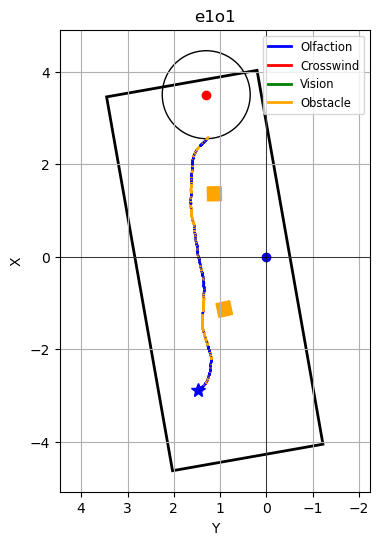
\includegraphics[width=0.2\columnwidth]{Main/Figure/e1o1.png}\label{fig:e1o1}}
    \subfigure[e1o2]{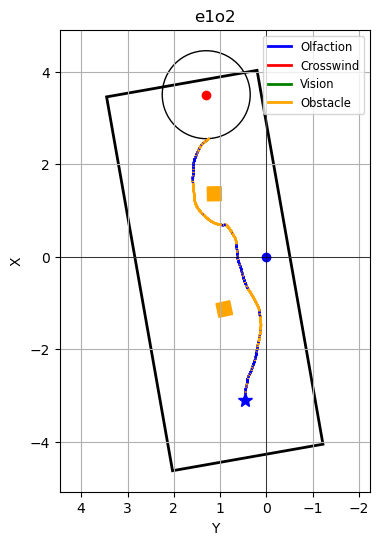
\includegraphics[width=0.2\columnwidth]{Main/Figure/e1o2.png}\label{fig:e1o2}}
    \subfigure[e1o3]{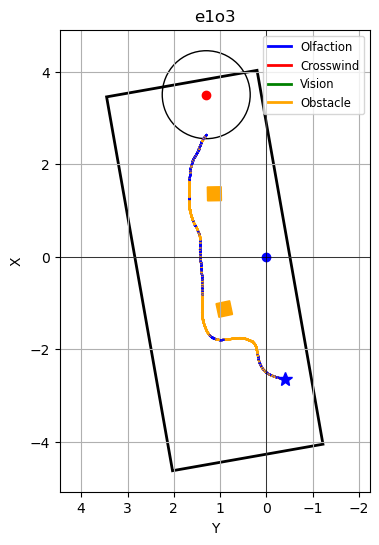
\includegraphics[width=0.2\columnwidth]{Main/Figure/e1o3.png}\label{fig:e1o3}}
    \subfigure[e1o4]{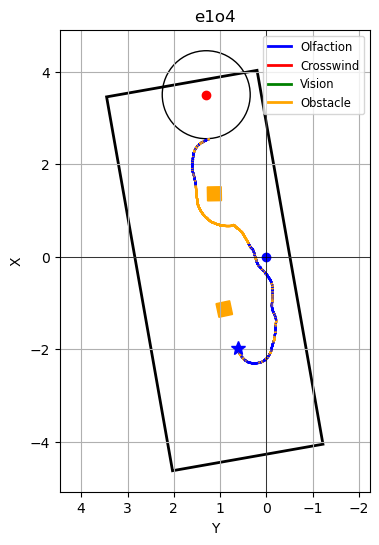
\includegraphics[width=0.2\columnwidth]{Main/Figure/e1o4.png}\label{fig:e1o4}}
    \subfigure[e1o5]{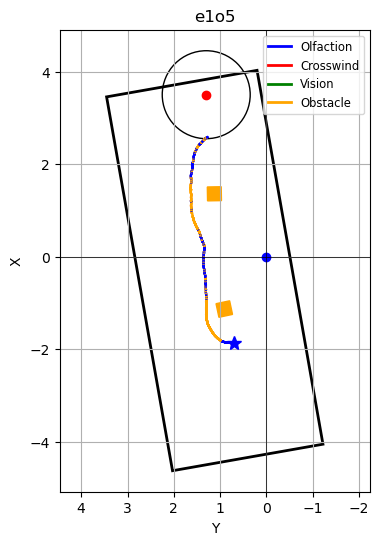
\includegraphics[width=0.2\columnwidth]{Main/Figure/e1o5.png}\label{fig:e1o5}}
    \subfigure[e2o1]{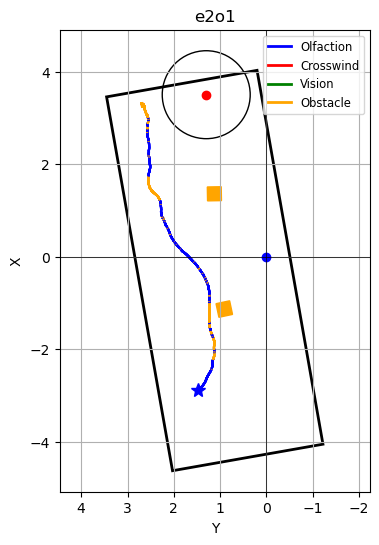
\includegraphics[width=0.2\columnwidth]{Main/Figure/e2o1.png}\label{fig:e2o1}}
    \subfigure[e2o2]{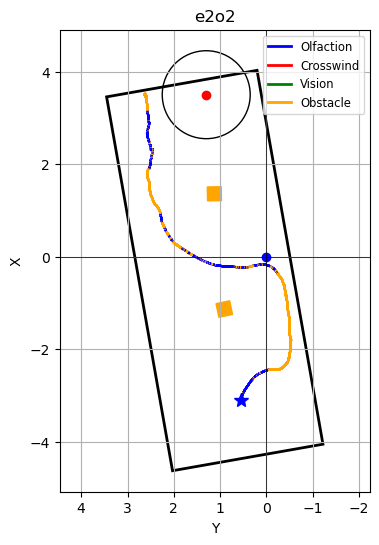
\includegraphics[width=0.2\columnwidth]{Main/Figure/e2o2.png}\label{fig:e2o2}}
    \subfigure[e2o3]{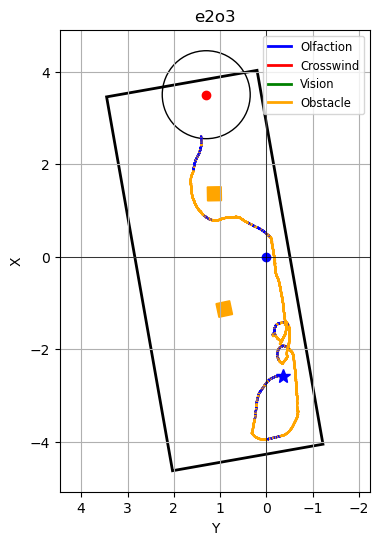
\includegraphics[width=0.2\columnwidth]{Main/Figure/e2o3.png}\label{fig:e2o3}}
    \subfigure[e2o4]{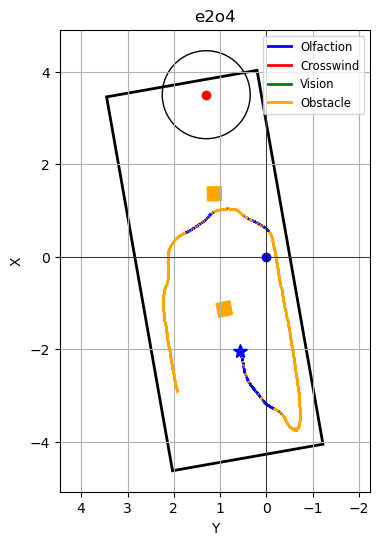
\includegraphics[width=0.2\columnwidth]{Main/Figure/e2o4.png}\label{fig:e2o4}}
    \subfigure[e2o5]{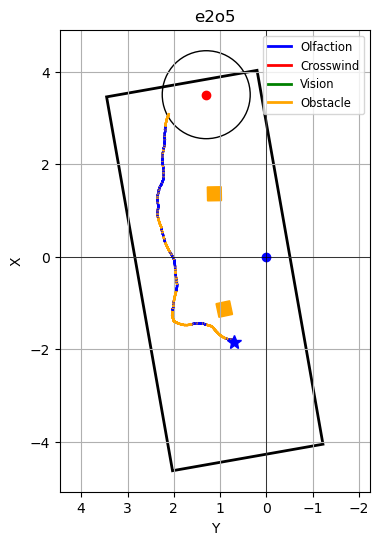
\includegraphics[width=0.2\columnwidth]{Main/Figure/e2o5.png}\label{fig:e2o5}}
\end{center}
\vspace{-.1in}

\caption
{Trajectories of OSL repeat experiments. Olfaction-only Navigation algorithm trials (o1-o5) in - (1-5) laminar airflow environment (e1), and (6-10) turbulent airflow environment (e2). The behaviors that the robot was following under the three navigation algorithms are Crosswind - crosswind maneuver behavior, Obstacle - Obstacle-avoid Navigation behavior, Olfaction - Olfaction-based Navigation behavior, and Vision - Vision-based Navigation behavior. Robot starting positions are highlighted with a blue star, the obstacles are the orange boxes, and the odor source is the red point with the surrounding circular source declaration region.}
%\end{singlespace}
\label{fig:individualTrajectoriesOO}
\end{figure}




\begin{figure}[h!] %% figure

\ \\
\vspace*{-.18in}

\begin{center}
    \subfigure[e1v1]{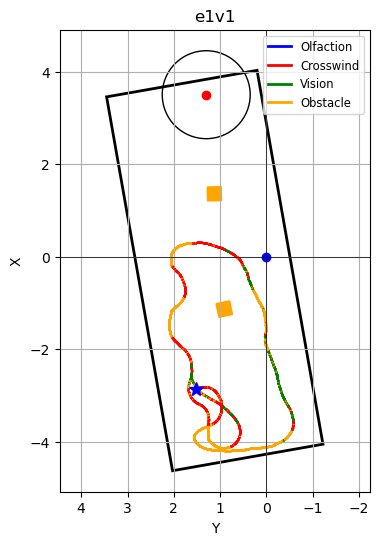
\includegraphics[width=0.2\columnwidth]{Main/Figure/e1v1.png}\label{fig:e1v1}}
    \subfigure[e1v2]{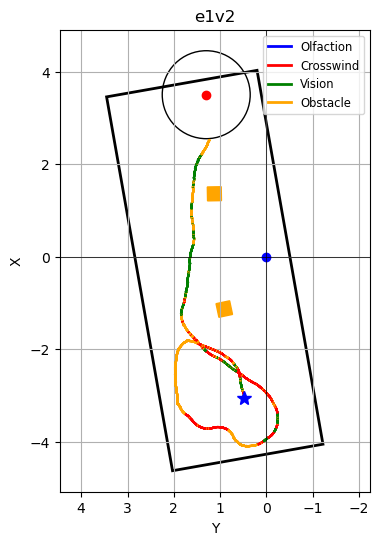
\includegraphics[width=0.2\columnwidth]{Main/Figure/e1v2.png}\label{fig:e1v2}}
    \subfigure[e1v3]{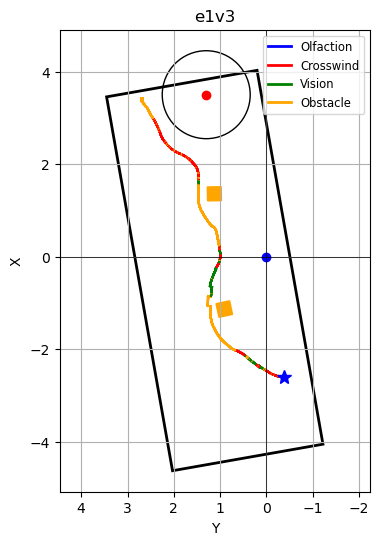
\includegraphics[width=0.2\columnwidth]{Main/Figure/e1v3.png}\label{fig:e1v3}}
    \subfigure[e1v4]{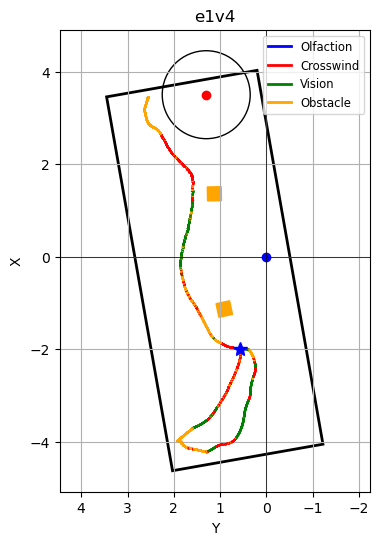
\includegraphics[width=0.2\columnwidth]{Main/Figure/e1v4.png}\label{fig:e1v4}}
    \subfigure[e1v5]{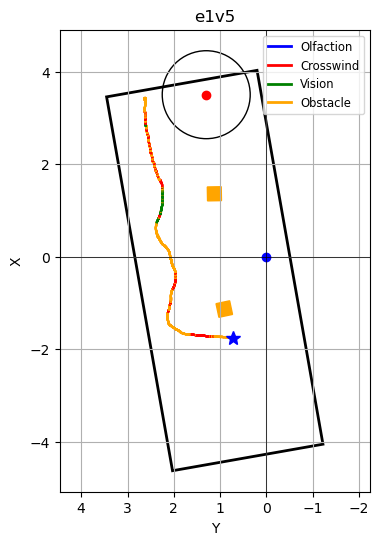
\includegraphics[width=0.2\columnwidth]{Main/Figure/e1v5.png}\label{fig:e1v5}}
    \subfigure[e2v1]{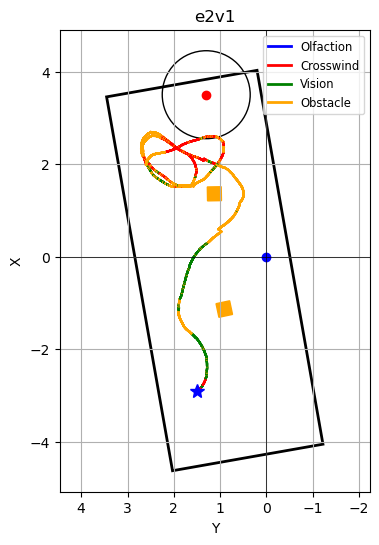
\includegraphics[width=0.2\columnwidth]{Main/Figure/e2v1.png}\label{fig:e2v1}}
    \subfigure[e2v2]{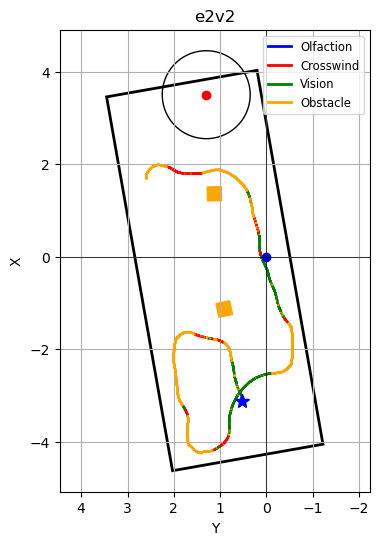
\includegraphics[width=0.2\columnwidth]{Main/Figure/e2v2.png}\label{fig:e2v2}}
    \subfigure[e2v3]{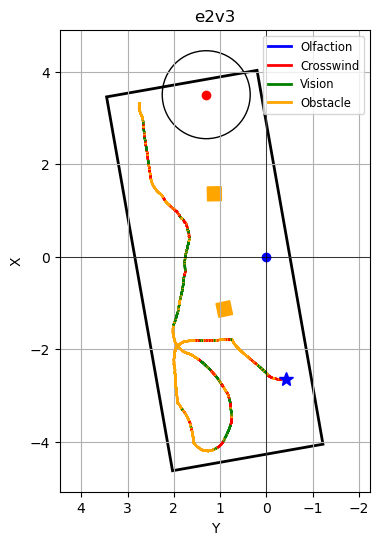
\includegraphics[width=0.2\columnwidth]{Main/Figure/e2v3.png}\label{fig:e2v3}}
    \subfigure[e2v4]{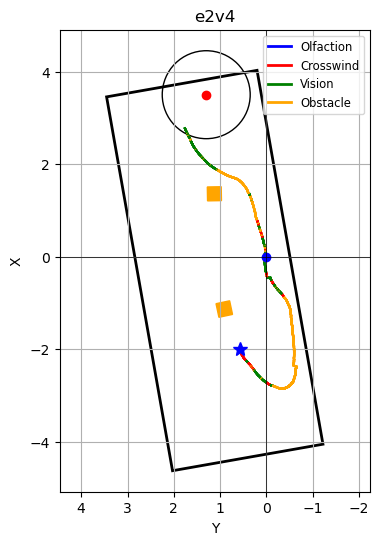
\includegraphics[width=0.2\columnwidth]{Main/Figure/e2v4.png}\label{fig:e2v4}}
    \subfigure[e2v5]{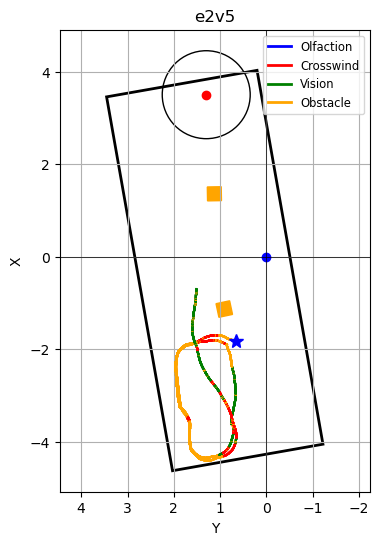
\includegraphics[width=0.2\columnwidth]{Main/Figure/e2v5.png}\label{fig:e2v5}}
\end{center}
\vspace{-.1in}

\caption
{Trajectories of OSL repeat experiments. Vision-only Navigation algorithm trials in - (1-5) laminar airflow environment (e1), and (6-10) turbulent airflow environment (e2). The behaviors that the robot was following under the three navigation algorithms are Crosswind - crosswind maneuver behavior, Obstacle - Obstacle-avoid Navigation behavior, Olfaction - Olfaction-based Navigation behavior, and Vision - Vision-based Navigation behavior. Robot starting positions are highlighted with a blue star, the obstacles are the orange boxes, and the odor source is the red point with the surrounding circular source declaration region.}
%\end{singlespace}
\label{fig:individualTrajectoriesVO}
\end{figure}



\begin{figure}[h!] %% figure

\ \\
\vspace*{-.18in}

\begin{center}
    \subfigure[e1vo1]{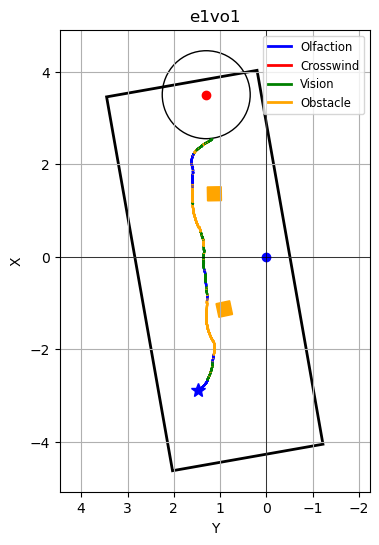
\includegraphics[width=0.2\columnwidth]{Main/Figure/e1ov1.png}\label{fig:e1vo1}}
    \subfigure[e1vo2]{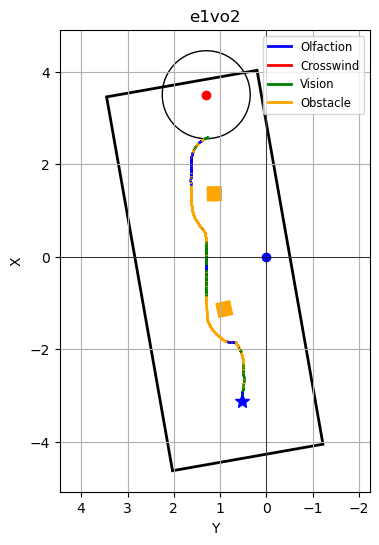
\includegraphics[width=0.2\columnwidth]{Main/Figure/e1ov2.png}\label{fig:e1vo2}}
    \subfigure[e1vo3]{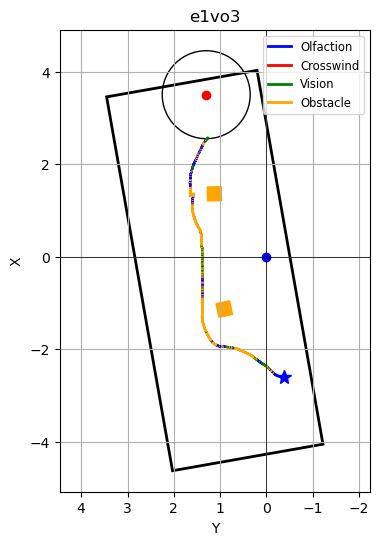
\includegraphics[width=0.2\columnwidth]{Main/Figure/e1ov3.png}\label{fig:e1vo3}}
    \subfigure[e1vo4]{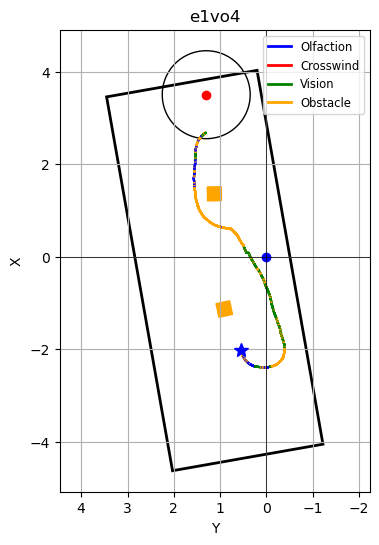
\includegraphics[width=0.2\columnwidth]{Main/Figure/e1ov4.png}\label{fig:e1vo4}}
    \subfigure[e1vo5]{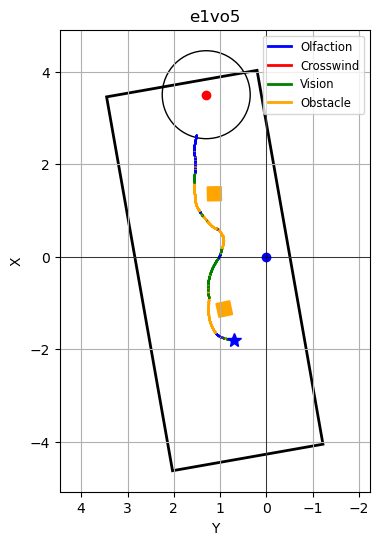
\includegraphics[width=0.2\columnwidth]{Main/Figure/e1ov5.png}\label{fig:e1vo5}}
    \subfigure[e2vo1]{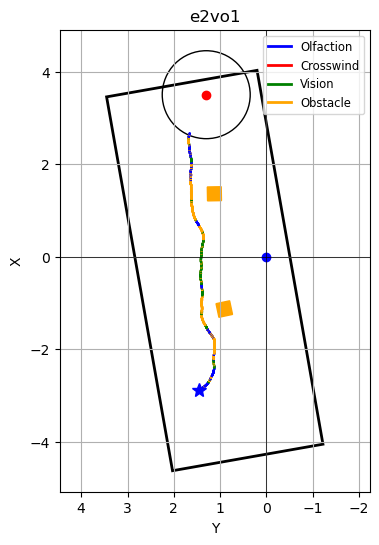
\includegraphics[width=0.2\columnwidth]{Main/Figure/e2ov1.png}\label{fig:e2vo1}}
    \subfigure[e2vo2]{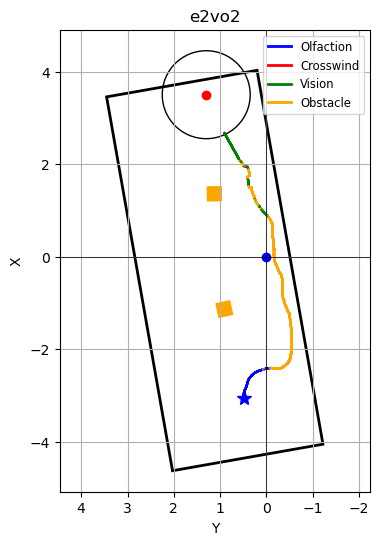
\includegraphics[width=0.2\columnwidth]{Main/Figure/e2ov2.png}\label{fig:e2vo2}}
    \subfigure[e2vo3]{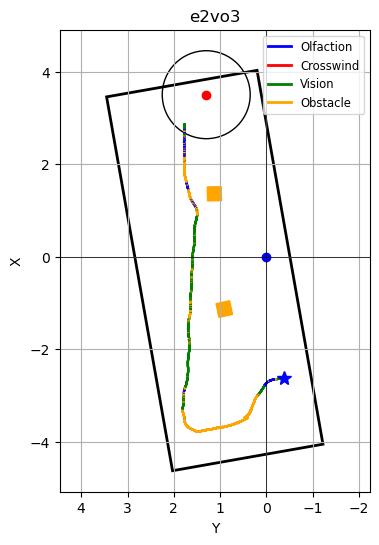
\includegraphics[width=0.2\columnwidth]{Main/Figure/e2ov3.png}\label{fig:e2vo3}}
    \subfigure[e2vo4]{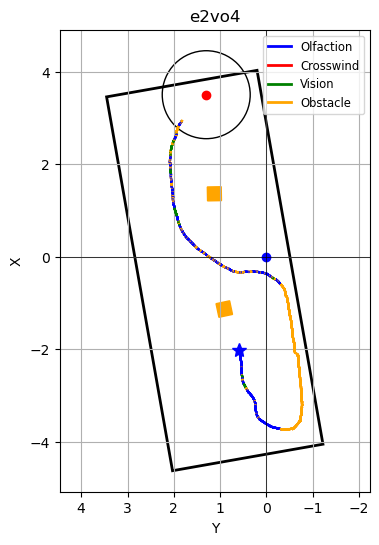
\includegraphics[width=0.2\columnwidth]{Main/Figure/e2ov4.png}\label{fig:e2vo4}}
    \subfigure[e2vo5]{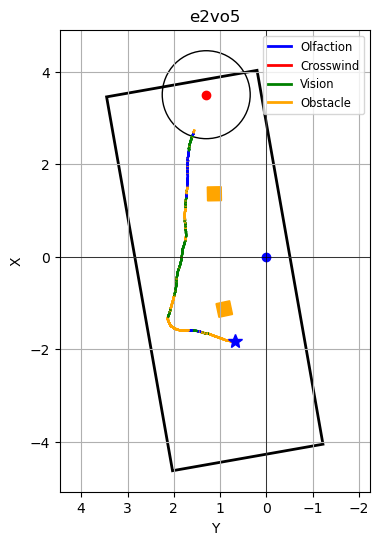
\includegraphics[width=0.2\columnwidth]{Main/Figure/e2ov5.png}\label{fig:e2vo5}}
\end{center}
\vspace{-.1in}

\caption
{Trajectories of OSL repeat experiments. Vision and Olfaction Fusion Navigation algorithm trials (o1-o5) in - (1-5) laminar airflow environment (e1), and (6-10) turbulent airflow environment (e2). The behaviors that the robot was following under the three navigation algorithms are Crosswind - crosswind maneuver behavior, Obstacle - Obstacle-avoid Navigation behavior, Olfaction - Olfaction-based Navigation behavior, and Vision - Vision-based Navigation behavior. Robot starting positions are highlighted with a blue star, the obstacles are the orange boxes, and the odor source is the red point with the surrounding circular source declaration region.}
%\end{singlespace}
\label{fig:individualTrajectoriesFusion}
\end{figure}
\end{comment}

\begin{figure}[h!] %% figure
\ \\
\vspace*{-.18in}
\begin{center}
    \subfigure[e1o]{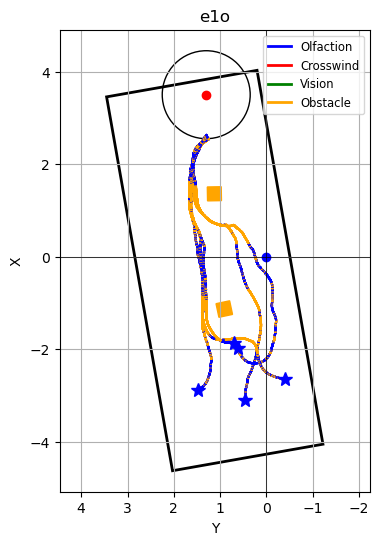
\includegraphics[width=0.3\columnwidth]{Main/Figure/e1o.png}\label{fig:e1o}}
    \subfigure[e1v]{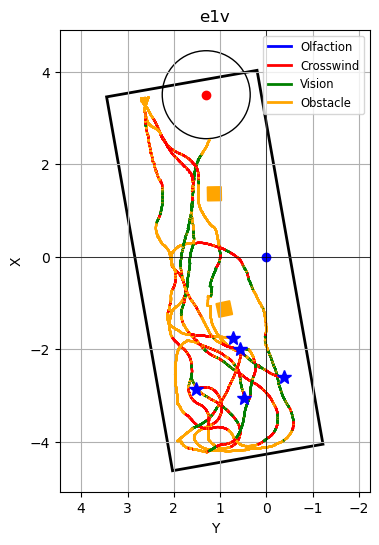
\includegraphics[width=0.3\columnwidth]{Main/Figure/e1v.png}\label{fig:e1v}}
    \subfigure[e1vo]{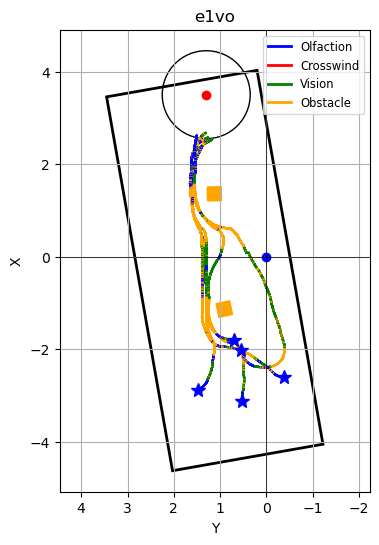
\includegraphics[width=0.3\columnwidth]{Main/Figure/e1ov.png}\label{fig:e1vo}}
    \subfigure[e2o]{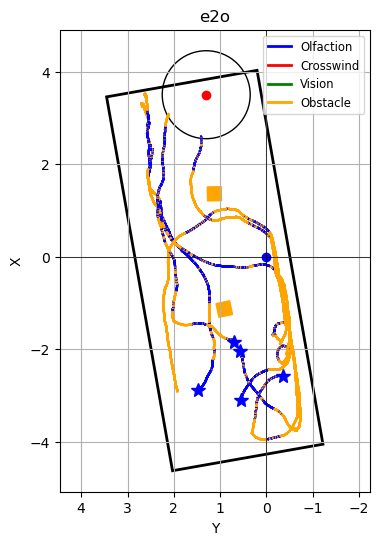
\includegraphics[width=0.3\columnwidth]{Main/Figure/e2o.png}\label{fig:e2o}}
    \subfigure[e2v]{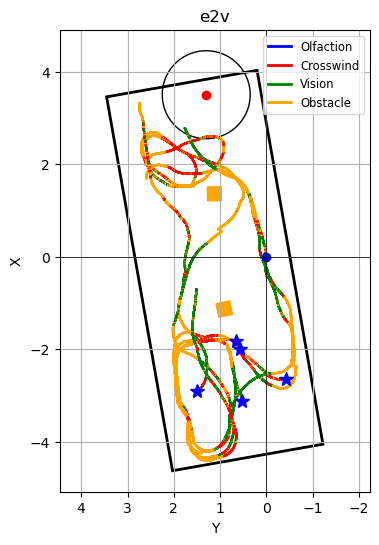
\includegraphics[width=0.3\columnwidth]{Main/Figure/e2v.png}\label{fig:e2v}}
    \subfigure[e2vo]{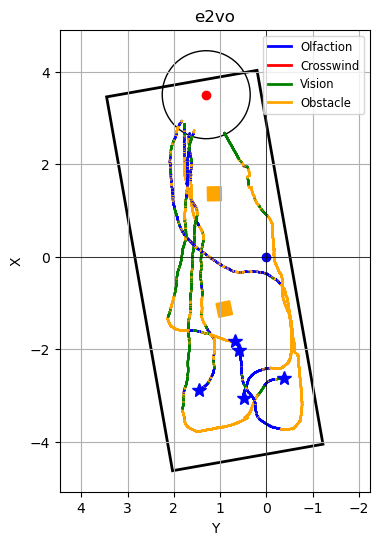
\includegraphics[width=0.3\columnwidth]{Main/Figure/e2ov.png}\label{fig:e2vo}}
\end{center}
\vspace{-.1in}

\caption
{Robot trajectories of repeated tests in six navigation algorithm and airflow environment combinations. Trajectories in laminar airflow environments are (a) e1o—Olfaction-Only Navigation algorithm, (b) e1v—Vision-Only Navigation algorithm, and (c) e1vo—Vision and Olfaction Fusion Navigation algorithm. Trajectories in turbulent airflow environments are (d) e2o—Olfaction-Only Navigation algorithm, (e) e2v—Vision-Only Navigation algorithm, and (f) e2vo—Vision and Olfaction Fusion Navigation algorithm. The 1behaviors the robot followed: Crosswind maneuver behavior, Obstacle-Avoid behavior, Olfaction-Based behavior, and Vision-Based behavior. Five robot starting positions are marked with a blue star, obstacles are indicated by orange boxes, and the odor source is represented by a red point with the surrounding circular source declaration region.}
%\end{singlespace}
\label{fig:combinedTrajectories}
\end{figure}

Table~\ref{tab:expeiment_result} presents the run times for the 30 trial runs, consisting of 5 trials using each of the 3 navigation algorithms in the 2 airflow environments. %Figure~\ref{fig:individualTrajectoriesOO}, Figure~\ref{fig:individualTrajectoriesVO}, and Figure~\ref{fig:individualTrajectoriesFusion} illustrate the robot trajectories for each of the 30 trial runs.
Figure~\ref{fig:combinedTrajectories} shows the combined robot trajectories for the three navigation algorithms across the two airflow environments. Table~\ref{tab:expeiment_stat} summarizes the repeated test results, detailing success rate, average search time, and average distance traveled. The results indicate that the proposed Vision and Olfaction Fusion Navigation algorithm achieves the highest success rate, the lowest average search time, and the shortest average distance traveled among the three methods. This is crucial for real-world odor source localization applications, where it is essential for the robot to locate odor sources as quickly as possible.


The Olfaction-Only Navigation algorithm utilizes airflow direction to guide the robot toward the odor source. It performed well in laminar airflow environments, with the robot following relatively direct airflow paths to the odor source. However, in turbulent airflow environments, the robot was often diverted by complex airflow patterns and frequently failed to reach the odor source within the designated time limit.

Vision-Based Navigation performed poorly in both laminar and turbulent airflow environments. Due to the placement of obstacles, the robot had no initial vision of the plume from the starting position. It had to rely on Crosswind maneuver and Obstacle-Avoid Navigation behaviors until it obtained a valid plume visual. In most runs, the 200 s time limit expired before the robot could locate and navigate to the odor source.

The Vision and Olfaction Fusion Navigation algorithm test runs consistently succeeded in both laminar and turbulent airflow environments. The Crosswind maneuver and Olfaction-Based Navigation directed the robot toward the odor source, enabling it to detect the plume visually. Once the robot switched to Vision-Based Navigation, it was no longer affected by turbulent airflow.

